%versi 3 (22-07-2020)
\chapter{Perancangan}
\label{chap:perancangan}

Pada bab ini akan dijelaskan mengenai perancangan aplikasi yang akan dibangun meliputi perancangan kelas pada masing-masing komponen beserta dengan deskripsi dan fungsinya, dan perancangan struktur HTML. Untuk antarmuka pada aplikasi yang akan dibangun akan memiliki antarmuka yang sama dengan aplikasi WSDC 2017 Bali terdahulu. Penjelasan terkait dengan antarmuka telah dibahas pada bagian~\ref{sec:StrukturIonic3SistemKini}. 

\section{Perancangan Kelas}
\label{sec:perancanganKelas}

Pada aplikasi WSDC 2017 Bali yang akan dibangun menggunakan struktur kelas yang sama dengan aplikasi WSDC 2017 Bali terdahulu, dengan beberapa penyesuaian terkait dengan pembaruan yang dilakukan. Diagram kelas secara keseluruhan dapat dilihat pada~gambar~\ref{fig:umldiagramkeseluruhan}.

\begin{figure}[H]
    \centering
    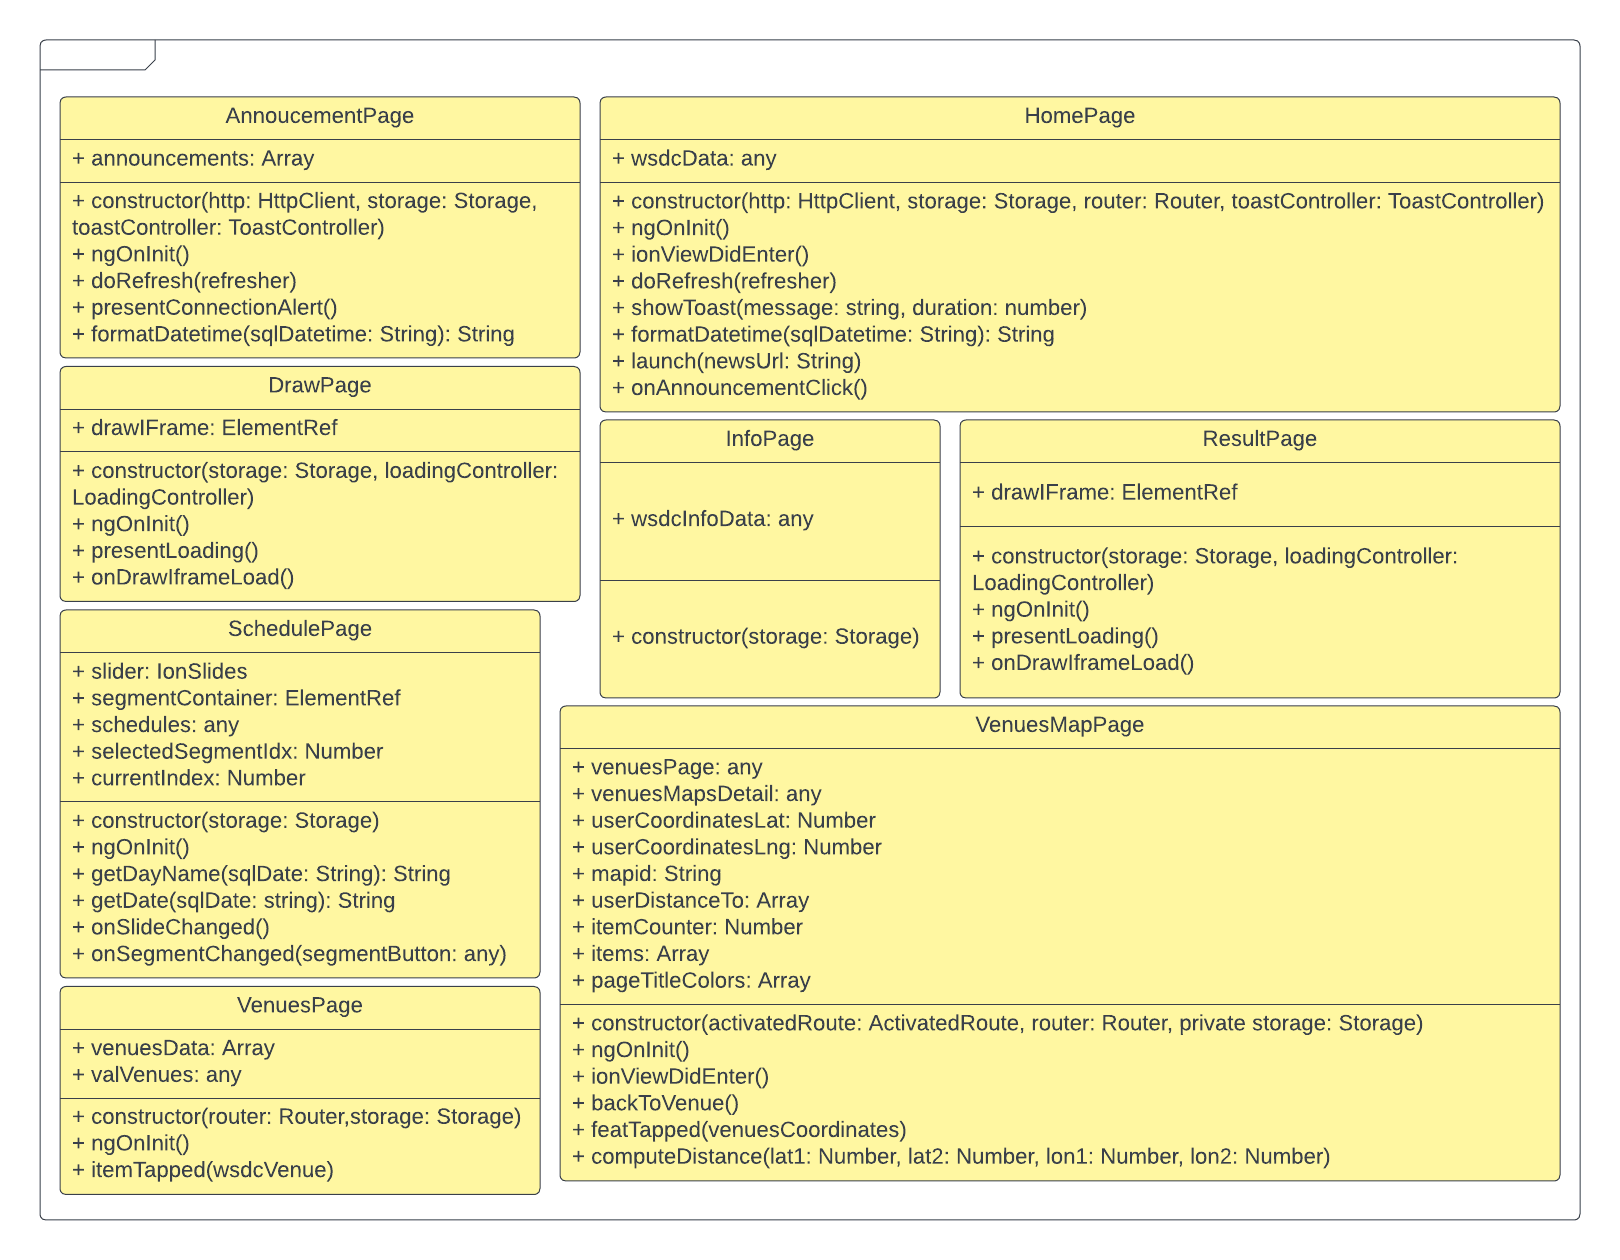
\includegraphics[scale=0.25]{Gambar/umldiagram.png}
    \caption{ Diagram Kelas Keseluruhan}
    \label{fig:umldiagramkeseluruhan}
\end{figure}

\newpage

Perancangan kelas dari masing-masing komponen adalah sebagai berikut:

\begin{enumerate}
	\item Komponen \textit{Announcements} \\
	Di dalam komponen \textit{announcements} terdapat sebuah kelas AnnouncementPage. Kelas ini berfungsi untuk mengambil data \textit{announcements} 	dari \textit{storage}, dan menampilkan pengumuman ke halaman \textit{announcements}. Kelas ini memiliki sebuah atribut, yaitu announcements bertipe \textit{array} yang menyimpan localtime bertipe data \textit{string} yang berisi tanggal dan waktu dari sebuah pengumuman dikeluarkan dengan format ``Tahun-Bulan-Hari Jam:Menit:Detik'', dan message yang berisi pesan pengumuman yang bertipe data \textit{string}. 
	Kelas ini memiliki beberapa \textit{method}, diantaranya adalah sebagai berikut:
	
	\begin{itemize}
		\item \textbf{constructor(private http: HttpClient, private storage: Storage, public toastController: ToastController)}\\
		\textit{Method} constructor berfungsi untuk memberikan nilai awal pada saat kelas dibuat.
		\textbf{Parameter}: 
		\begin{itemize}
			\item \textbf{http}: Parameter ini digunakan untuk menyimpan API HttpClient.
			\item \textbf{storage}: Parameter ini digunakan untuk menyimpan API Storage.
			\item \textbf{toastController}: Parameter ini digunakan untuk menyimpan API ToastController.
		\end{itemize}
		\textbf{Kembalian}; tidak ada.	
		
		\item \textbf{ngOnInit()}\\
		\textit{Method} ini berfungsi untuk mengambil data \textit{announcements} yang terdapat di dalam \textit{storage}, kemudian menyimpannya ke dalam atribut kelas, yaitu announcements. \\
		\textbf{Parameter}: tidak ada. \\
		\textbf{Kembalian}: tidak ada.	
		
		\item \textbf{doRefresh(refresher)} \\
		\textit{Method} ini berfungsi untuk melakukan penyegaran ulang terhadap halaman \textit{Announcements}. Saat melakukan penyegaran ulang, \textit{method} ini akan mengambil data terbaru dari server, kemudian menyimpannya ke dalam atribut kelas, yaitu announcements. Selanjutnya akan dilakukan penghapusan terlebih dahulu terhadap data yang sudah ada di dalam \textit{storage}, kemudian menyimpan data terbaru yang di dapatkan dari server ke dalam \textit{storage}. Jika server tidak merespon dan data tidak dapat diambil, maka akan memanggil \textit{method} presentConnectionAlert() untuk menampilkan \textit{toast}. \\
		\textbf{Parameter}: \textit{Method} ini memiliki sebuah parameter yaitu refresher, yang berisi \textit{event refresher}.\\
		\textbf{Kembalian}: tidak ada.
		
		\item \textbf{presentConnectionAlert()} \\
		\textit{Method} ini berfungsi untuk menampilkan \textit{toast} yang akan menamipilkan sebuah tulisan ``Failed to refresh information'' selama tiga detik. \textit{Method} ini hanya akan digunakan ketika \textit{method} doRefresh tidak berhasil mengambil data terbaru dari server.\\
		\textbf{Parameter}: tidak ada.\\
		\textbf{Kembalian}: tidak ada.
		\newpage
		\item \textbf{formatDatetime(sqlDatetime: string)} \\
		\textit{Method} ini berfungsi untuk mengambil jam, menit, hari, dan bulan dari parameter. \\
		\textbf{Parameter}: sqlDatetime: detail waktu dan tanggal pada sebuah pengumuman. \\
		\textbf{Kembalian}: sebuah \textit{string} yang berisi tanggal dan waktu dari sebuah pengumuman dengan format ``Jam-Menit | Hari, Tanggal, Bulan''.
	\end{itemize}
	
	\item Komponen \textit{Draw} \\
	Di dalam komponen \textit{announcements} terdapat sebuah kelas DrawPage. Kelas ini berfungsi untuk mengambil data \textit{draw} dari \textit{storage}, serta menampilkan data \textit{draw} ke halaman \textit{draw}. Kelas ini memiliki sebuah atribut, yaitu drawIFrame yang bertipe ElementRef. Atribut ini merupakan sebuah ViewChild yang digunakan untuk memanggil elemen dari komponen \textit{draw}, yaitu drawIFrame pada \textit{file} draw.page.html. 
	
	Kelas ini memiliki beberapa \textit{method}, diantaranya adalah sebagai berikut:
	
	\begin{itemize}
		\item \textbf{constructor(private storage: Storage,public loadingController: LoadingController)}\\
			\textit{Method} constructor berfungsi untuk memberikan nilai awal pada saat kelas dibuat.
			\textbf{Parameter}:
			\begin{itemize}
				\item \textbf{storage}: Parameter ini digunakan untuk menyimpan API Storage.
				\item \textbf{loadingController}: Parameter ini digunakan untuk menyimpan API LoadingController.
			\end{itemize}
			\textbf{Kembalian}: tidak ada.

		\item \textbf{ngOnInit()} \\
			\textit{Method} ini berfungsi untuk mengambil data \textit{draws} yang terdapat di dalam \textit{storage}. Data tersebut lalu disimpan ke dalam \textit{child} drawIFrame. Kemudian \textit{method} ini akan memanggil \textit{method} presentLoading(). \\
			\textbf{Parameter}: tidak ada. \\
			\textbf{Kembalian}: tidak ada.
		
		\item \textbf{async presentLoading()}\\
			\textit{Method} ini berfungsi untuk menampilkan sebuah indikator \textit{loading} dengan pesan ``Please wait...''. \\ 
			\textbf{Parameter}: tidak ada. \\
			\textbf{Kembalian}: tidak ada.
			
		\item \textbf{onDrawIframeLoad()}\\
			\textit{Method} ini merupakan sebuah \textit{template statement} yang dipanggil oleh \textit{event} di dalam \textit{tag} \texttt{<iframe>} pada \textit{file} draw.page.html. \textit{Method} ini berfungsi untuk menampilkan data \textit{draw} yang disimpan di dalam \textit{storage}. \\
			\textbf{Parameter}: tidak ada. \\
			\textbf{Kembalian}: tidak ada.
	\end{itemize}
	
	\item Komponen \textit{Home} \\
	Di dalam komponen \textit{home} terdapat sebuah kelas HomePage. Kelas ini menjadi sebagai kelas yang pertama kali diakses oleh aplikasi. Maka dari itu, kelas ini berfungsi untuk menginisialisasi sebuah \textit{storage} yang diisi oleh data yang digunakan oleh seluruh kelas pada aplikasi. Kelas ini memiliki sebuah atribut, yaitu wsdcData yang bertipe any. Atribut ini akan menyimpan data json berisi data yang akan digunakan untuk aplikasi. 
	
	Kelas ini memiliki beberapa \textit{method}, diantaranya adalah sebagai berikut:
	
	\begin{itemize}
		\item \textbf{constructor(private http: HttpClient, private storage: Storage, private router: Router, public toastController: ToastController)} \\
			\textit{Method} constructor berfungsi untuk memberikan nilai awal pada saat kelas dibuat.
			\textbf{Parameter}:
			\begin{itemize}
				\item \textbf{http}: Parameter ini digunakan untuk menyimpan API HttpClient.
				\item \textbf{storage}: Parameter ini digunakan untuk menyimpan API Storage.
				\item \textbf{router}: Parameter ini digunakan untuk menyimpan API Router.
				\item \textbf{toastController}: Parameter ini digunakan untuk menyimpan API ToastController.
			\end{itemize}
			\textbf{Kembalian}: tidak ada.
		
		\item \textbf{ionViewDidEnter()}\\
			\textit{Method} ini dijalankan ketika halaman sudah masuk sepenuhnya. \textit{Method} ini berfungsi untuk menutup \textit{splash screen}. \\
			\textbf{Parameter}: tidak ada. \\
			\textbf{Kembalian}: tidak ada.
			
		\item \textbf{ngOnInit()} \\
			\textit{Method} ini berfungsi untuk mengambil data json dari \textit{storage}. Jika data di dalam \textit{storage} tersebut belum pernah dibuat sebelumnya, maka \textit{method} ini akan membuat sebuah data baru di dalam \textit{storage} yang berisi data json yang dibutuhkan untuk aplikasi. Secara \textit{default}, untuk mengantisipasi jika pengguna tidak memiliki koneksi internet, maka pertama kali \textit{method} ini mengambil data adalah dari aset yang berada di \textit{folder} assets. Setelah itu, \textit{method} ini akan mengambil data terbaru dari server. Jika server tidak merespon dan data tidak berhasil didapatkan, maka akan memanggil \textit{method} showToast(). \\
			\textbf{Parameter}: tidak ada. \\
			\textbf{Kembalian}: tidak ada.
			
		\item \textbf{doRefresh(refresher)} \\
			\textit{Method} ini berfungsi untuk melakukan penyegaran ulang terhadap halaman \textit{Home}. Saat melakukan penyegaran ulang, \textit{method} ini akan mengambil data terbaru dari server, kemudian menyimpannya ke dalam atribut kelas, yaitu wsdcData. Selanjutnya akan dilakukan penghapusan terlebih dahulu terhadap data yang sudah ada di dalam \textit{storage}, kemudian menyimpan data terbaru yang di dapatkan dari server ke dalam \textit{storage}. Jika server tidak memberi respon dan data tidak dapat diambil, maka akan memanggil \textit{method} showToast() untuk menampilkan \textit{toast}. \\
			\textbf{Parameter}: tidak ada. \\
			\textbf{Kembalian}: tidak ada.
			
		\item \textbf{async showToast(message: string, duration: number=3000)}\\
			\textit{Method} ini berfungsi untuk menampilkan \textit{toast} yang akan menampilkan pesan dan durasi sesuai dengan yang ada pada parameter.\\
			\newpage
			\textbf{Parameter}:
			\begin{itemize}
				\item \textbf{message}: pesan yang akan ditampilkan di dalam \textit{toast}.
				\item \textbf{duration}: durasi seberapa lama \textit{toast} berada di layar.
			\end{itemize}
			\textbf{Kembalian}: tidak ada.
			
		\item \textbf{formatDatetime(sqlDatetime: string)}\\
			\textit{Method} ini berfungsi untuk mengambil jam, menit, hari, dan bulan dari parameter. \\\
			\textbf{Parameter}: sqlDatetime: detail waktu dan tanggal pada sebuah pengumuman. \\
			\textbf{Kembalian}: sebuah \textit{string} yang berisi tanggal dan waktu dari sebuah pengumuman dengan format ``Hari | Jam-Menit''.
			
		\item \textbf{launch(newsUrl: string)}\\
			\textit{Method} ini berfungsi untuk membuka url berita sesuai dengan url yang ada di dalam parameter. \\
			\textbf{Parameter}: newsUrl: \textit{string} url dari sebuah berita. \\
			\textbf{Kembalian}: tidak ada.
			
		\item \textbf{onAnnouncementClick()} \\
			\textit{Method} ini berfungsi untuk berpindah halaman ke halaman \textit{announcements}.\\
			\textbf{Parameter}: tidak ada.\\
			\textbf{Kembalian}: tidak ada.
	\end{itemize}
	
	
	\item Komponen Info \\
		Di dalam komponen info terdapat sebuah kelas InfoPage. Kelas ini berfungsi untuk mengambil data info dari \textit{stroage} dan menyimpannya ke atriubt kelas yang kemudian data tersebut akan ditampilkan ke halaman info. Kelas ini memiliki sebuah atribut, yaitu wsdcInfoData yang bertipe any. Atribut ini digunakan untuk menyimpan data untuk halaman info. Kelas ini hanya memiliki sebuah \textit{method} yaitu \textit{method} constructor. \textit{Method} ini memiliki sebuah parameter, yaitu storage yang bertipe Storage. Constructor pada kelas ini bertujuan untuk mengambil data info dari \textit{storage} dan menyimpannya ke dalam atribut kelas, yaitu wsdcInfoData. 
		
	\item Komponen \textit{Result} \\
		Di dalam komponen \textit{result} terdapat sebuah kelas ResultPage. Kelas ini berfungsi untuk mengambil data \textit{result} dari \textit{storage} yang kemudian data tersebut akan ditampilkan ke halaman \textit{result}. Kelas ini memiliki sebuah atribut yaitu resultIFrame yang bertipe ElementRef. Atribut ini merupakan sebuah @ViewChild yang digunakan untuk memanggil elemen dari komponen \textit{result}, yaitu resultIFrame pada \textit{file} result.page.html. 
		
		Kelas ini memiliki beberapa \textit{method}, diantaranya adalah sebagai berikut:
		
		\begin{itemize}
			\item \textbf{constructor(private storage: Storage,public loadingController: LoadingController)} \\ 
				\textit{Method} constructor berfungsi untuk memberikan nilai awal pada saat kelas dibuat.
				\textbf{Parameter}:
				\begin{itemize}
					\item \textbf{storage}: Parameter ini digunakan untuk menyimpan API Storage.
					\item \textbf{loadingController}: Parameter ini digunakan untuk menyimpan API LoadingController.
				\end{itemize}
				\textbf{Kembalian}: tidak ada.
			\newpage
			\item \textbf{ngOnInit()}\\ 
				\textit{Method} ini berfungsi untuk mengambil data \textit{result} yang terdapat di dalam \textit{storage}. Data tersebut lalu disimpan ke dalam \textit{child} resultIFrame. Setelah itu \textit{method} ini akan memanggil \textit{method} presentLoading(). \\
				\textbf{Parameter}: tidak ada. \\
				\textbf{Kembalian}: tidak ada.
				
			\item \textbf{async presentLoading()}\\
				\textit{Method} ini berfungsi untuk menampilkan sebuah indikator \textit{loading} dengan pesan ``Please wait...''. \\ 
				\textbf{Parameter}: tidak ada. \\
				\textbf{Kembalian}: tidak ada.
				
			\item \textbf{onResultIframeLoad()} \\
				\textit{Method} ini merupakan sebuah \textit{template statement} yang dipanggil oleh \textit{event} di dalam \textit{tag} \texttt{<iframe>} pada \textit{file} result.page.html. \textit{Method} ini berfungsi untuk menampilkan data \textit{result} yang disimpan di dalam \textit{storage}. \\
				\textbf{Parameter}: tidak ada. \\
				\textbf{Kembalian}: tidak ada.
		\end{itemize}


		\item Komponen \textit{Schedule}\\
			Di dalam komponen \textit{schedule} terdapat sebuah kelas SchedulePage. Kelas ini berfungsi untuk mengatur jadwal pada halaman \textit{schedule}, seperti mengatur perpindahan \textit{slides} dan \textit{segment} pada jadwal. 

			Kelas ini memiliki beberapa atribut, diantaranya adalah sebagai berikut:
			\begin{itemize} 
				\item \textbf{slider}: Atribut ini merupakan sebuah @ViewChild yang digunakan untuk memanggil elemen dari komponen \textit{schedule}, yaitu scheduleSlider pada \textit{file} schedule.page.html.
				\item \textbf{segmentContainer}: Atribut ini merupakan sebuah @ViewChild yang digunakan untuk memanggil elemen dari komponen \textit{schedule}, yaitu segmentContainer pada \textit{file} schedule.page.html.
				\item \textbf{schedules}: Atribut ini akan menyimpan data \textit{schedules} yang diambil dari \textit{storage}.
				\item \textbf{slideOpts}: Atriubt ini berisi pengaturan dasar untuk \textit{slides}. Berisi initialSlide untuk mengatur \textit{slides} ke berapa saat pertama kali halaman \textit{schedule} dibuka, dan \textit{speed} untuk mengatur kecepatan transisi antar \textit{slides}.
				\item \textbf{selectedSegmentIdx}: Atribut ini digunakan untuk menyimpan index dari \textit{segment} yang sedang aktif.
				\item \textbf{currentIndex}: Atribut ini digunakan untuk menyimpan index dari \textit{slides} yang sedang aktif.
			\end{itemize}
			Kelas ini memiliki beberapa \textit{method}, diantaranya adalah sebagai berikut:
			\begin{itemize}
				\item \textbf{constructor(private storage: Storage)}\\ 
					\textit{Method} constructor berfungsi untuk memberikan nilai awal pada saat kelas dibuat. \\
					\textbf{Parameter}: storage: Parameter ini digunakan untuk menyimpan API Storage.\\
					\textbf{Kembalian}: tidak ada.
					\newpage
					
				\item \textbf{ngOnInit()}\\ 
				\textit{Method} ini berfungsi untuk mengambil data \textit{schedule} yang terdapat di dalam \textit{storage}. Data tersebut lalu disimpan ke dalam atribut \textit{schedules}. \\
				\textbf{Parameter}: tidak ada. \\
				\textbf{Kembalian}: tidak ada.
				
				\item \textbf{getDayName(sqlDate: string)}\\
					\textit{Method} ini berfungsi untuk mengambil hari dari parameter. \\
					\textbf{Parameter}: sqlDate: Sebuah \textit{string} yang berisi tahun, bulan, dan tanggal.\\
					\textbf{Kembalian}: \textit{string} nama hari.
				
				\item \textbf{getDate(sqlDate: string)}\\
					\textit{Method} ini berfungsi untuk mengambil tanggal dari parameter. \\
					\textbf{Parameter}: sqlDate: Sebuah \textit{string} yang berisi tahun, bulan, dan tanggal. \\
					\textbf{Kembalian}: \textit{string} tanggal.
					
				\item \textbf{onSlideChanged()}\\
					\textit{Method} ini dipanggil saat \textit{slides} dipindahkan dengan cara digeser ke kanan atau ke kiri. \textit{Method} ini akan mengubah atribut currentIndex menjadi index \textit{slides} saat ini, kemudian mengubah atribud selectedSegmentIdx menjadi index \textit{slides} saat ini. Hal ini bertujuan agar indeks dari \textit{segment} yang aktif dapat diganti sesuai dengan indeks \textit{slides} yang aktif. Dengan begitu tampilan \textit{segment} dan \textit{slides} yang aktif akan sesuai. \\
					\textbf{Parameter}: tidak ada. \\
					\textbf{Kembalian}: tidak ada.
									
					
				\item \textbf{onSegmentChanged(segmentButton)}\\
					\textit{Method} ini berfungsi untuk mengubah \textit{slides} yang aktif sesuai dengan indeks dari \textit{segment} yang sedang aktif. \\
					\textbf{Parameter}: segmentButton: Merupakan sebuah \textit{event} dari \textit{segment} yang akan diambil \textit{value} yang berisi indeks dari \textit{segment} yang aktif. \\
					\textbf{Kembalian}: tidak ada.
			\end{itemize}
			
			\item Komponen \textit{Venues} \\
				Di dalam komponen \textit{venues} terdapat sebuah kelas VenuesPage. Kelas ini berfungsi untuk mengambil data \textit{venues} dari \textit{storage} dan menyimpannya ke dalam atribut kelas. Selain itu kelas ini juga berfungsi melakukan navigasi ke halaman \textit{venues map}.
				
				Kelas ini memiliki beberapa atribut, yaitu:
				\begin{itemize}
					\item \textbf{venuesData}: Atribut ini bertipe array. Atribut ini digunakan untuk menyimpan data dari \textit{venues} yang berisi id, name, icon, geojson, dan colorIdx dari masing masing kategori \textit{venues}. Data ini nantinya akan dikirimkan ke kelas \textit{Venues Maps}.
					\item \textbf{valVenues}: Digunakan untuk menyimpan data \textit{venues} yang didapatkan dari \textit{storage}.
				\end{itemize}
				
				Kelas ini memiliki beberapa \textit{method}, diantaranya yaitu:
				\begin{itemize}
					\item \textbf{constructor(private router: Router,private storage: Storage)}\\ 
						\textit{Method} constructor berfungsi untuk memberikan nilai awal pada saat kelas dibuat. \\
						\newpage
						\textbf{Parameter}: 
						\begin{itemize}
							\item \textbf{router}: Parameter ini berfungsi untuk menyimpan API Router.
							\item \textbf{storage}: Parameter ini berfungsi untuk menyimpan API Storage.
						\end{itemize}
						\textbf{Kembalian}: tidak ada.
						
					\item \textbf{ngOnInit()}\\ 
					\textit{Method} ini berfungsi untuk mengambil data \textit{venues} yang terdapat di dalam \textit{storage}. Data tersebut lalu disimpan ke dalam atribut \textit{valVenues}. \\
					\textbf{Parameter}: tidak ada. \\
					\textbf{Kembalian}: tidak ada.
						
					\item \textbf{itemTapped(wsdcVenue)} \\
						\textit{Method} ini berfungsi untuk melakuakn navigasi ke halaman \textit{Venues Maps} dengan bantuan Router milik Angular. \textit{Method} ini akan mengirimkan sebuah data array yang didapatkan dari parameter ke halaman \textit{Venues Maps}. \\
						\textbf{Parameter}: wsdcVenue: Parameter ini merupakan sebuah array yang berisi sama seperti atribut venuesData. Isi dari array ini adalah data untuk sebuah \textit{venues} yang ingin dilihat. \\
						\textbf{Kembalian}: tidak ada.
				\end{itemize}
				
			\item Komponen \textit{Venues Maps}\\ 
				Di dalam komponen \textit{venues Maps} terdapat sebuah kelas VenuesMapsPage. Kelas ini berfungsi untuk mengambil data \textit{venues} yang dikirimkan dari komponen \textit{Venues}, menampilkan peta \textit{venues}, serta melakukan kalkulasi jarak pengguna dengan \textit{venues}. Kelas ini memiliki beberapa atribut, yaitu:
				
				\begin{itemize}
					\item \textbf{venuesPage} : Atribut ini digunakan untuk menyimpan data yang dikirimkan dari komponen \textit{Venues}.
					\item \textbf{venuesMapsDetail} : Atribut ini digunakan untuk menyimpan data \textit{venues} dari \textit{storage} sesuai dengan kategori yang sedang dipilih.
					\item \textbf{userCoordinatesLat} : Atirbut ini digunakan untuk menyimpan koordinat latitude dari perangkat pengguna.
					\item \textbf{userCoordinatesLng} : Atirbut ini digunakan untuk menyimpan koordinat longitude dari perangkat pengguna.
					\item \textbf{mapid} : Atribut ini digunakan untuk menyimpan id dari peta.
					\item \textbf{userDistanceTo} : Atribut ini digunakan untuk menyimpan jarak dari posisi perangkat pengguna ke posisi \textit{venues}.
					\item \textbf{itemCounter} : Atribut ini digunakan sebagai penghitung berapa banyak \textit{venues} dalam sebuah kategori.
					\item \textbf{items} : Atribut ini digunakan untuk menyimpan id dan id warna dari sebuah kategori~\textit{venues}.
					\item \textbf{pageTitleColors} : Atribut ini merupakan sebuah \textit{array}~yang~berisi~kode~warna~untuk~masing-masing~judul kategori~\textit{venues}.
				\end{itemize} 
				Kelas ini memiliki beberapa \textit{method}, diantaranya adalah sebagai berikut:
				\begin{itemize}
					\item \textbf{constructor(private activatedRoute: ActivatedRoute, private router: Router, private storage: Storage)} \\
					\newpage
						\textit{Method} constructor berfungsi untuk memberikan nilai awal pada saat kelas dibuat. Selain itu, \textit{constructor} juga digunakan untuk mengambil data dari \textit{storage} dan memasukannya ke atribut venuesMapsDetail.\\
						\textbf{Parameter}:
						\begin{itemize}
							\item \textbf{activatedRoute} : Parameter ini digunakan untuk menyimpan API ActivatedRoute.
							\item \textbf{router} : Parameter ini digunakan untuk menyimpan API Router.
							\item \textbf{storage} : Parameter ini digunakan untuk menyimpan API Storage.
						\end{itemize}
						\textbf{Kembalian}: tidak ada.
						
					\item \textbf{ngOnInit()}\\ 
					\textit{Method} ini berfungsi untuk mengambil data \textit{venues} yang terdapat di dalam \textit{storage}. Data tersebut lalu disimpan ke dalam atribut \textit{venuesMapsDetail}. \\
					\textbf{Parameter}: tidak ada. \\
					\textbf{Kembalian}: tidak ada.
						
					\item \textbf{ionViewDidEnter()} \\
						\textit{Method} ini dijalankan ketika halaman sudah masuk sepenuhnya. \textit{Method} ini digunakan untuk menginisialisasi peta menggunakan \textit{plugin} Google Maps yang disediakan oleh Capacitor. Peta tersebut menampilkan peta Pulau Bali, lebih tepatnya di Kecamatan Kuta dengan latitude -8.722396 dan longitude 115.17671. \textit{Method} ini juga membuat \textit{marker} yang menandai setiap lokasi \textit{venues} pada satu kategori \textit{venues}. Selain itu \textit{method} ini juga digunakan untuk menyimpan jarak antara posisi perangkat pengguna ke masing-masing posisi \textit{venues}, yang kemudian disimpan ke dalam atibut userDistanceTo.\\
						\textbf{Parameter}: tidak ada. \\
						\textbf{Kembalian}: tidak ada.
						
					\item \textbf{backToVenue()} \\
						\textit{Method} ini digunakan untuk bernavigasi kembali ke halaman \textit{Venues}. \\
						\textbf{Parameter}: tidak ada. \\
						\textbf{Kembalian}: tidak ada.
						
					\item \textbf{featTapped(venuesCoordinates)} \\
						\textit{Method} ini digunakan untuk mengarahkan kamera map ke arah lokasi \textit{venues} yang dituju sesuai dengan koordinat pada parameter. \\
						\textbf{Parameter}: venuesCoordinates: Parameter ini berisi koordinat latitude dan longitude dari lokasi \textit{venues} yang dituju. \\
						\textbf{Kembalian}: tidak ada.
						
					\item \textbf{computeDistance(lat1, lat2, lon1, lon2)} \\
						\textit{Method} ini berfungsi untuk menghitung jarak dari posisi perangkat pengguna ke posisi \textit{venues} menggunakan latitude dan longitude dari kedua posisi tersebut.\\
						\textbf{Parameter}: 
						\begin{itemize}
							\item \textbf{lat1}: koordinat latitude dari pengguna.
							\item \textbf{lat2}: koordinat latitude dari \textit{venues}.
							\item \textbf{lon1}: koordinat longitude dari pengguna.
							\item \textbf{lon2}: koordinat longitude dari \textit{venues}.
						\end{itemize}
						\textbf{Kembalian}: \textit{String} jarak~dari~posisi~perangkat~pengguna~ke~posisi~\textit{venues}.
				\end{itemize}
\end{enumerate}

\section{Perancangan Struktur HTML}
\label{sec:perancanganStrukturHTML}

	Struktur HTML pada masing-masing komponen mengambil struktur yang sama dengan aplikasi WSDC 2017 Bali terdahulu, namun dengan beberapa perubahan. Perubahan-perubahan tersebut telah dibahas pada bagian~\ref{subsec:migrasi}, serta analisis penggunaannya di sistem usulan pada bagian~\ref{sec:analisisKebutuhanSistem}.
	
	Masing-masing HTML yang terdapat pada setiap komponen memiliki struktur yang sama, yaitu terdapat sebuah \textit{header} dan sebuah \textit{content}. Penjelasan struktur pada \textit{header} dan \textit{content} adalah sebagai berikut:
	
	\begin{enumerate}
		\item \textit{Header} \\
			\textit{Header} untuk setiap komponen pada umunya memiliki struktur yang serupa namun dibedakan dengan judul dari setiap halaman. \textit{Header} digunakan untuk menampilkan judul dari sebuah halaman, serta menyediakan sebuah \textit{menu button} sebagai salah satu cara untuk membuat \textit{sidemenu} untuk melakukan navigasi antar halaman. \textit{Header} dibungkus oleh \textit{tag} \texttt{<ion-header>} yang didalamnya terdapat \textit{tag} \texttt{<ion-toolbar>} yang disediakan Ionic Framework. Kemudian untuk \textit{menu button} dibuat oleh \textit{tag} \texttt{<ion-menu-button>} pada \textit{tag} \texttt{<ion-buttons>}. Selanjutnya untuk judul dari sebuah halaman dibungkus oleh \textit{tag} \texttt{<ion-title>}. Judul akan berbeda beda tergantung dengan halamannya. Salah satu contoh dari penggunaan \textit{header} adalah pada gambar~\ref{fig:homePageWireframe} yang ditandai dengan kotak berwarna biru.
			
		\item \textit{Content} \\
			\textit{Content} untuk setiap komponen memiliki struktur yang berbeda-beda tergantung dengan isi dari halaman tersebut. Namun \textit{content} untuk setiap komponen dibungkus oleh sebuah \textit{tag} \texttt{<ion-content>}. Salah satu contoh dari penggunaan \textit{content} adalah pada gambar~\ref{fig:homePageWireframe} yang ditandai dengan warna merah. Struktur \textit{content} untuk masing-masing halaman adalah sebagai berikut:
			
			\begin{itemize}
				\item Halaman \textit{Announcements} \\
					\textit{Content} pada halaman \textit{announcements} berisi sebuah \textit{refresher} dengan \textit{tag} \texttt{<ion-refresher>} untuk melakukan penyegaran ulang terhadap halaman \textit{announcements} yaitu mengambil data terbaru dari server. Penggunaan \textit{tag} \texttt{<ion-refresher>} seperti pada gambar~\ref{fig:announcementsPageWireframe} yang ditandai dengan kotak berwarna hijau. Selain itu terdapat sebuah list dengan \textit{tag} \texttt{<ion-list>} yang ditandai dengan kotak berwarna kuning. List menampilkan pengumuman yang berisi waktu dan tanggal, serta pesan dari pengumuman tersebut. Setiap satu pengumuman dibungkus oleh sebuah \textit{tag} \texttt{<ion-item>} yang ditandai dengan kotak berwarna hitam. Di dalamnya terdapat sebuah \textit{tag} \texttt{<ion-label>} yang berisi \textit{tag} \texttt{<h3>} untuk waktu dan tanggal, serta \textit{tag} \texttt{<p>} untuk pesan pengumuman.		
				
				\item Halaman \textit{Draw} \\
					\textit{Content} pada halaman \textit{draw} berisi sebuah \textit{tag} \texttt{<iframe>} yang digunakan untuk menyematkan dokumen lain ke dalam dokumen HTML, yaitu sebuah data \textit{draw} yang berisi pembagian grup proposisi dan oposisi bagi setiap negara peserta WSDC 2017 Bali. Data tersebut diambil dari server, kemudian dimasukan ke dalam \textit{tag} \texttt{<iframe>}. Penggunaan \textit{tag} \texttt{<iframe>} seperti pada gambar~\ref{fig:drawPageWireframe} yang ditandai dengan kotak berwarna hijau.
					
				\item Halaman \textit{Home} \\
					\textit{Content} pada halaman \textit{home} berisi sebuah \textit{refresher} dengan \textit{tag} \texttt{<ion-refresher>} untuk melakukan penyegaran ulang terhadap halaman \textit{home}, yaitu mengambil data terbaru dari server. Penggunaan \textit{tag} \texttt{<ion-refresher>} seperti pada gambar~\ref{fig:homePageWireframe} yang ditandai dengan kotak berwarna hijau. Selain itu terdapat sebuah \textit{card} dengan \textit{tag} \texttt{<ion-card>} seperti yang ditandai dengan kotak berwarna merah muda yang digunakan untuk menampilkan sebuah pengumuman terbaru, berikut dengan waktu dan tanggal serta pesan dari pengumuman tersebut. Di dalam \textit{card} terdapat \textit{grid} untuk \textit{layout} dari \textit{card}. Di dalam sebuah \textit{grid} terdapat sebuah baris dengan \textit{tag} \texttt{<ion-row>}. Di dalam baris tersebut terdapat dua buah kolom dengan \textit{tag} \texttt{<ion-col>}. Masing-masing kolom memiliki ukuran, kolom pertama yang ditandai dengan kotak berwarna coklat berukuran sembilan digunakan untuk menyimpan \textit{header} dari \textit{card} dengan \textit{title} yaitu ``Latest Announcement''. \textit{Header} ini dibungkus di dalam \textit{tag} \texttt{<ion-card-header>}, dan \textit{title} dengan \textit{tag} \texttt{<ion-card-title>}. Selain \textit{header} untuk \textit{card}, terdapat pula \textit{content} untuk \textit{card} dengan \textit{tag} \texttt{<ion-card-content>} yang berisi waktu dan tanggal, serta pesan dari pengumuman. Untuk kolom selanjutnya dengan ukuran tiga berisi sebuah gambar seperti yang ditandai dengan kotak berwarna jingga.
					
					Selain \textit{card} pengumuman, terdapat juga list dengan \textit{tag} \texttt{<ion-list>} yang berisi \textit{thumbnail} dari berita-berita terkait acara WSDC 2017 Bali seperti yang ditandai dengan kotak berwarna ungu pada gambar~\ref{fig:homePageWireframe}. Di dalam list terdapat sebuah \textit{header} dengan \textit{tag} \texttt{<ion-list-header>} yang berisi judul dari list yaitu ``Newsletters'' yang berada di dalam \textit{tag} \texttt{<ion-label>}. Untuk masing-masing \textit{thumbnail} berita berada di dalam \textit{tag} \texttt{<ion-item>}. Untuk masing-masing item terdapat sebuah gambar \textit{thumbnail} dari sebuah berita, judul dari berita tersebut, serta sebuah tombol dengan \textit{tag} \texttt{<ion-button>} yang jika ditekan akan mengarahkan pengguna untuk melihat berita tertentu sesuai dengan item yang dipilih.
				
				\item Halaman Info \\
					\textit{Content} pada halaman info berisi sebuah \textit{grid} dengan \textit{tag} \texttt{<ion-grid>}, yang berisi sebuah baris dengan \textit{tag} \texttt{<ion-row>}. Baris ini menyimpan info-info seputar kontak-kontak penting yang dapat dihubungi, kosa kata dalam Bahasa Indonesia sehari-hari, serta credits kepada pembuat aplikasi WSDC 2017 Bali.
					
				\item Halaman \textit{Result}\\
					\textit{Content} pada halaman \textit{result} berisi sebuah \textit{tag} \texttt{<iframe>} yang digunakan untuk menyematkan dokumen lain ke dalam dokumen HTML, yaitu sebuah data \textit{result} hasil dari keseluruhan pertandingan WSDC 2017 Bali. Data tersebut diambil dari server, kemudian dimasukan ke dalam \textit{tag} \texttt{<iframe>}. 
					
				\item Halaman \textit{Schedule} \\
					\textit{Content} pada halaman \textit{schedule} berisi \textit{segment} dengan \textit{tag} \texttt{<ion-segment>} dan sebuah \textit{slides} dengan \textit{tag} \texttt{<ion-slides>}. \textit{Segment} digunakan untuk menampilkan tanggal dan hari, serta berfungsi untuk memindahkan \textit{slides} ke hari yang dipilih seperti yang ditandai dengan kotak berwarna hijau pada gambar~\ref{fig:SchedulePageWireframe}. Untuk melakukan hal tersebut, di dalam \textit{segment} terdapat sebuah \textit{button} dengan \textit{tag} \texttt{<ion-segment-button>} yang berisi \textit{tag} \texttt{<ion-label>} untuk menampung tanggal dan hari. 
					Sedangkan \textit{slides} digunakan untuk menampilkan jadwal acara WSDC 2017 Bali pada hari yang sesuai dengan \textit{segment} yang terpilih seperti yang ditandai dengan kotak berwarna coklat. Untuk menampilkan jadwal menggunakan \textit{list} dengan \textit{tag} \texttt{<ion-list>} yang ditandai dengan warna merah muda. Di dalam \textit{list} terdapat sebuah \textit{item} dengan \textit{tag} \texttt{<ion-item>}. Untuk setiap \textit{item} berisi waktu mulai dan selesai sebuah acara dengan \textit{tag} \texttt{<ion-note>} yang ditandai dengan warna ungu, serta nama acara dengan \textit{tag} \texttt{<h3>} yang ditandai dengan kotak berwarna jingga dan lokasi acara dengan \textit{tag} \texttt{<p>} yang ditandai dengan kotak berwarna biru muda. Nama dan lokasi acara dibungkus dengan \textit{tag} \texttt{<ion-label>}.
					
				\item Halaman \textit{Venues} \\
					\textit{Content} pada halaman \textit{venues} berisi \textit{grid} dengan \textit{tag} \texttt{<ion-grid>} dengan satu baris menggunakan \textit{tag} \texttt{<ion-row>}. Di dalamnya terdapat sebuah \textit{list} dengan \textit{tag} \texttt{<ion-list>}. \textit{List} tersebut berisi tombol dengan \textit{tag} \texttt{<ion-button>} yang ditandai dengan kotak berwarna hijau pada gambar~\ref{fig:VenuePageWireframe}. Masing-masing tombol digunakan untuk melakukan navigasi ke halaman \textit{venues map}. Setiap tombol berisi ikon dengan \textit{tag} \texttt{<ion-icon>} yang ditandai dengan kotak berwarna biru muda pada gambar~\ref{fig:VenuePageWireframe} dan sebuah \textit{tag} \texttt{<span>} yang berisi nama dari \textit{venues}, ditandai dengan kotak berwarna hitam.

				\item Halaman \textit{Venues Map} \\
					\textit{Content} pada halaman \textit{venues map} berisi \textit{tag} \texttt{<div>} yang digunakan untuk menampung peta dari sebuah kategori \textit{venues} seperti yang ditandai dengan kotak berwarna hijau pada gambar~\ref{fig:VenueMapPageWireframe}. Selain itu terdapat sebuah label dengan \textit{tag} \texttt{<ion-label>} yang berisi nama kategori \textit{venues} yang ditandai dengan kotak berwarna kuning. Kemudian untuk menampilkan nama dan deskripsi sebuah \textit{venues}, serta jarak antara pengguna dengan \textit{venues}, menggunakan \textit{list} dengan \textit{tag} \texttt{<ion-list>} yang ditandai dengan kotak berwarna biru muda. 
				
			\end{itemize}			  
	\end{enumerate}